\section{Training des Modells}
Ein zentraler Bestandteil des Projekts ist das Training eines eigenen Objekterkennungsmodells auf Basis von YOLO. 
Da die vortrainierten Modelle keine spezifischen Erkennungsobjekte wie Richtungspfeile umfassen, ist es erforderlich, ein benutzerdefiniertes Modell zu trainieren. 
Ziel des Trainingsprozesses ist es, das Modell so anzupassen, dass es die gewünschten Objekte zuverlässig und in Echtzeit erkennen kann.
\subsection{Aufnahme der Trainingsbilder}
Ein zentraler Bestandteil beim Training eines eigenen Objekterkennungsmodells ist die Erstellung eines passenden Datensatzes. 
Dabei kommt es nicht nur auf die Anzahl der Bilder an, sondern auch auf deren Vielfalt. 
Ziel ist es, das Modell möglichst gut auf die realen Einsatzbedingungen vorzubereiten. 
Daher sollten die Trainingsbilder unterschiedliche Perspektiven, Lichtverhältnisse, Objektgrößen und -anordnungen abdecken. 
Je abwechslungsreicher die Bilder, desto robuster wird das Modell gegenüber späteren Anwendungsszenarien.
\cite{yolo_data_docu}
\newPar
Für dieses Projekt wurden die Trainingsdaten aufgenommen, indem verschiedene Pfeile in unterschiedlichen Farben und Formen ausgedruckt und im Raum verteilt wurden. 
Die Anordnung und Orientierung der Pfeile wurde dabei bewusst variiert, mit teilweise bis zu zehn Pfeile auf einem Bild.
Die Fotos wurden mit einem handelsüblichen Smartphone aufgenommen, wobei wir verschiedene Blickwinkel gewählt haben, um eine möglichst breite Datenbasis zu schaffen. 
Insgesamt wurden dabei mehrere hundert Bilder erzeugt, in denen zusammen ca. tausend Pfeile zu sehen sind.
Diese Daten dienen als Grundlage für das nachfolgende Training des Modells.
\subsection{Vorverarbeitung und Labeling}
Für das Training von Objekterkennungsmodellen wie YOLO ist die Bildgröße ein wichtiger Faktor.
Modelle dieser Art erwarten in der Regel Eingabebilder mit festen Abmessungen, da neuronale Netze mit gleichbleibender Eingabegröße arbeiten.
\newPar
Im Projekt wurde sich für die Größe 640 x 480 Pixel entschieden, da mit entsprechend höherer Bildgröße auch der Speicher- und insbesondere der Rechenbedarf steigt.
Auch bei der Inferenz, also dem späteren Einsatz des trainierten Modells zur Objekterkennung, ist eine einheitliche Bildgröße erforderlich.
Die Eingabebilder werden dabei entweder im Vorfeld oder automatisch vom System auf die vom Modell erwartete Größe skaliert.
Es ist daher sinnvoll, die Bilder bereits vor oder während der Vorbereitung des Trainingsdatensatzes in das gewünschte Format zu bringen.
Als Vorverarbeitung der Traingsdaten wurden die Bilder daher auf eine Größe von 640 x 480 Pixel runterskaliert.
Dadurch konnte die Trainingszeit verkürzt und der Speicherbedarf reduziert werden. 
Ein Beispiel Trainingsbild ist in \imageref{beispiel_trainingsbild} dargestellt.
\cite{yolo_pre_docu}
\begin{figure}[H]
    \centering
    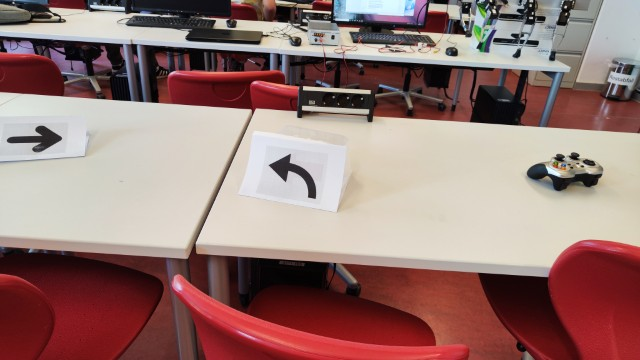
\includegraphics[width=0.75\linewidth]{example_image}
    \caption{Beispiel Trainings-Bild \textit{4f7e6590-88.jpg}}\label{beispiel_trainingsbild}
\end{figure}
Für den fertigen Trainings\hyp{}Datensatz wird zusätzlich zu den Bildern auch die dazugehörige Annotationsdatei benötigt. 
Diese enthalten Informationen über die Position und Klasse der Objekte im Bild, üblicherweise im sogenannten YOLO-Format.
Dieses speichert die Informationen in zwei Dateien, die jeweils den gleichen Dateinamen mit unterschiedlicher Endung aufweisen.
Das Bild an sich hat die entsprechende Bildformat-Endung, wie .jpg oder .png. Zusätzlich existiert eine Datei mit der Endung .txt, welche die Annotationen enthalten.
\cite{yolo_format_docu}
\newPar
Die zum Trainingsbild zugehörige Annotationsdatei \textit{4f7e6590-88.txt} sieht folgendermaßen aus:
\begin{lstlisting}
1 0.0552519011406844 0.3852978453738909
        0.09767110266159694 0.08365019011406837
0 0.4708606114138901 0.4680150843996924
        0.09415121255349486 0.1597717546362342
\end{lstlisting}

Dabei gibt die erste Zahl jeder Zeile die Klasse des Objektes und die nachfolgenden die Koordinaten der Bounding Box an.
\cite{yolo_format_docu}
\begin{figure}[H]
    \centering
    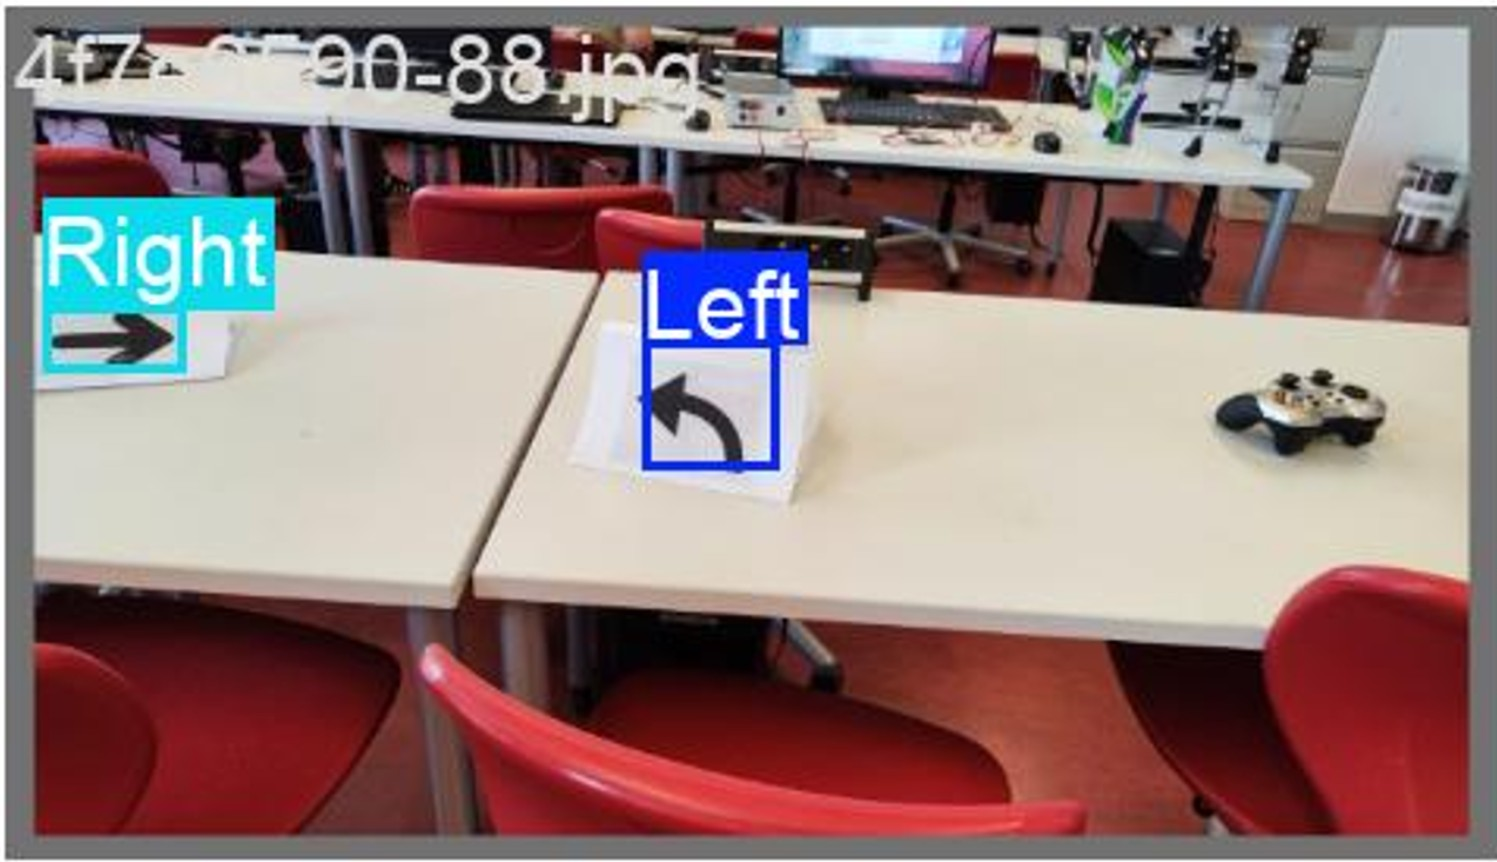
\includegraphics[width=0.8\linewidth]{example_labled}
    \caption{Beispiel gelabeltes Trainings-Bild}\label{beispiel_trainingsbild_labeld}
\end{figure}
Zusammengeführt sieht dieses Labelling dann entsprechend \imageref{beispiel_trainingsbild_labeld} aus.
Die Annotation der Daten kann mit speziellen Tools durchgeführt werden.
Im Projekt wurde dazu das Tool \gq{LabelStudio} von HumanSignal eingesetzt. Dieses stellt ein einfaches Web-Interface bereit, in dem das Labelling komfortabel vorgenommen werden kann.
\cite{labelstudio}
\subsection{Training}
Neben dem Datensatz selbst wird auch eine passende Trainingsumgebung benötigt. Dazu gehört Python als Programmiersprache sowie die Bibliothek PyTorch. 
Das eigentliche Training sollte mithilfe einer GPU erfolgen, da die Rechenprozesse sehr aufwendig sein können. Wichtig ist außerdem die Konfiguration des Modells und des Trainingsprozesses. 
Hierzu zählen unter anderem die Definition der Objektklassen und die Anzahl der Trainingsdurchläufe (Epochen).
\newPar
Für das Training des Modells wurde der aufbereitete Datensatz zunächst in Trainings\hyp{} und Validierungsdaten aufgeteilt. 
Dabei wurde ein klassisches 80/20\hyp{}Verhältnis gewählt, also 80\% der Bilder für das eigentliche Training und 20\% zur Validierung. 
Der Sinn dieser Aufteilung liegt darin, die Leistung des Modells nicht nur auf den gelernten Trainingsdaten zu beurteilen, sondern auch auf bisher \gq{unbekannten} Daten, 
um eine Überanpassung (das sogenannte Overfitting) zu vermeiden. 
Während des Trainings wird die Modellleistung regelmäßig mit den Validierungsdaten überprüft, wodurch die Modellqualität und der Lernfortschritt beurteilt werden kann.
\newPar
Das Training selbst wurde auf einem Laborrechner mit einer NVIDIA RTX 4060 Ti in der 16GB Variante durchgeführt. Es wurde keine feste Anzahl an Epochen vorgegeben. 
Stattdessen kam ein sogenanntes Early-Stopping-Verfahren zum Einsatz. Dabei wird das Training automatisch beendet, 
sobald sich die Modellleistung über einen bestimmten Zeitraum nicht mehr verbessert hat.
Dies wird, wie oben erläutert, anhand der Validierungsdaten gemessen. Im konkreten Fall wurde das Training nach etwa 300 Epochen abgebrochen. 
Eine Epoche dauerte durchschnittlich rund 800 Millisekunden, was zu einer Gesamttrainingszeit von etwa vier Minuten führte.
\newPar
Zum Vergleich: Ein Testlauf auf der virtuellen Maschine ohne GPU, also mit reinem CPU-Training, benötigte für das gleiche Training durch die deutlich schlechtere Performance und 
längere Reaktionszeit pro Epoche über eine Stunde. Dieser Vergleich unterstreicht den großen Einfluss der verwendeten Hardware auf die Effizienz und Praktikabilität des Trainingsprozesses. 
Besonders bei größeren Datensätzen oder komplexeren Modellen ist eine GPU-Unterstützung nahezu unerlässlich.
\newPar
An diesem Punkt wurde daher entschieden, die Inferenz und die Steuerung des Roboters aus Performancegründen auch auf den Laborrechner zu verschieben.
\subsection{Bewertung}
Zur Beurteilung des Modells können mehrere von PyTorch generierte Metriken betrachtet werden. Einen sehr guten, schnellen und einfach verständlichen Überblick bietet die sogenannte
Confusion-Matrix in \imageref{conf_matr} (hier in normalisierter Form).

\begin{figure}[H]
    \centering
    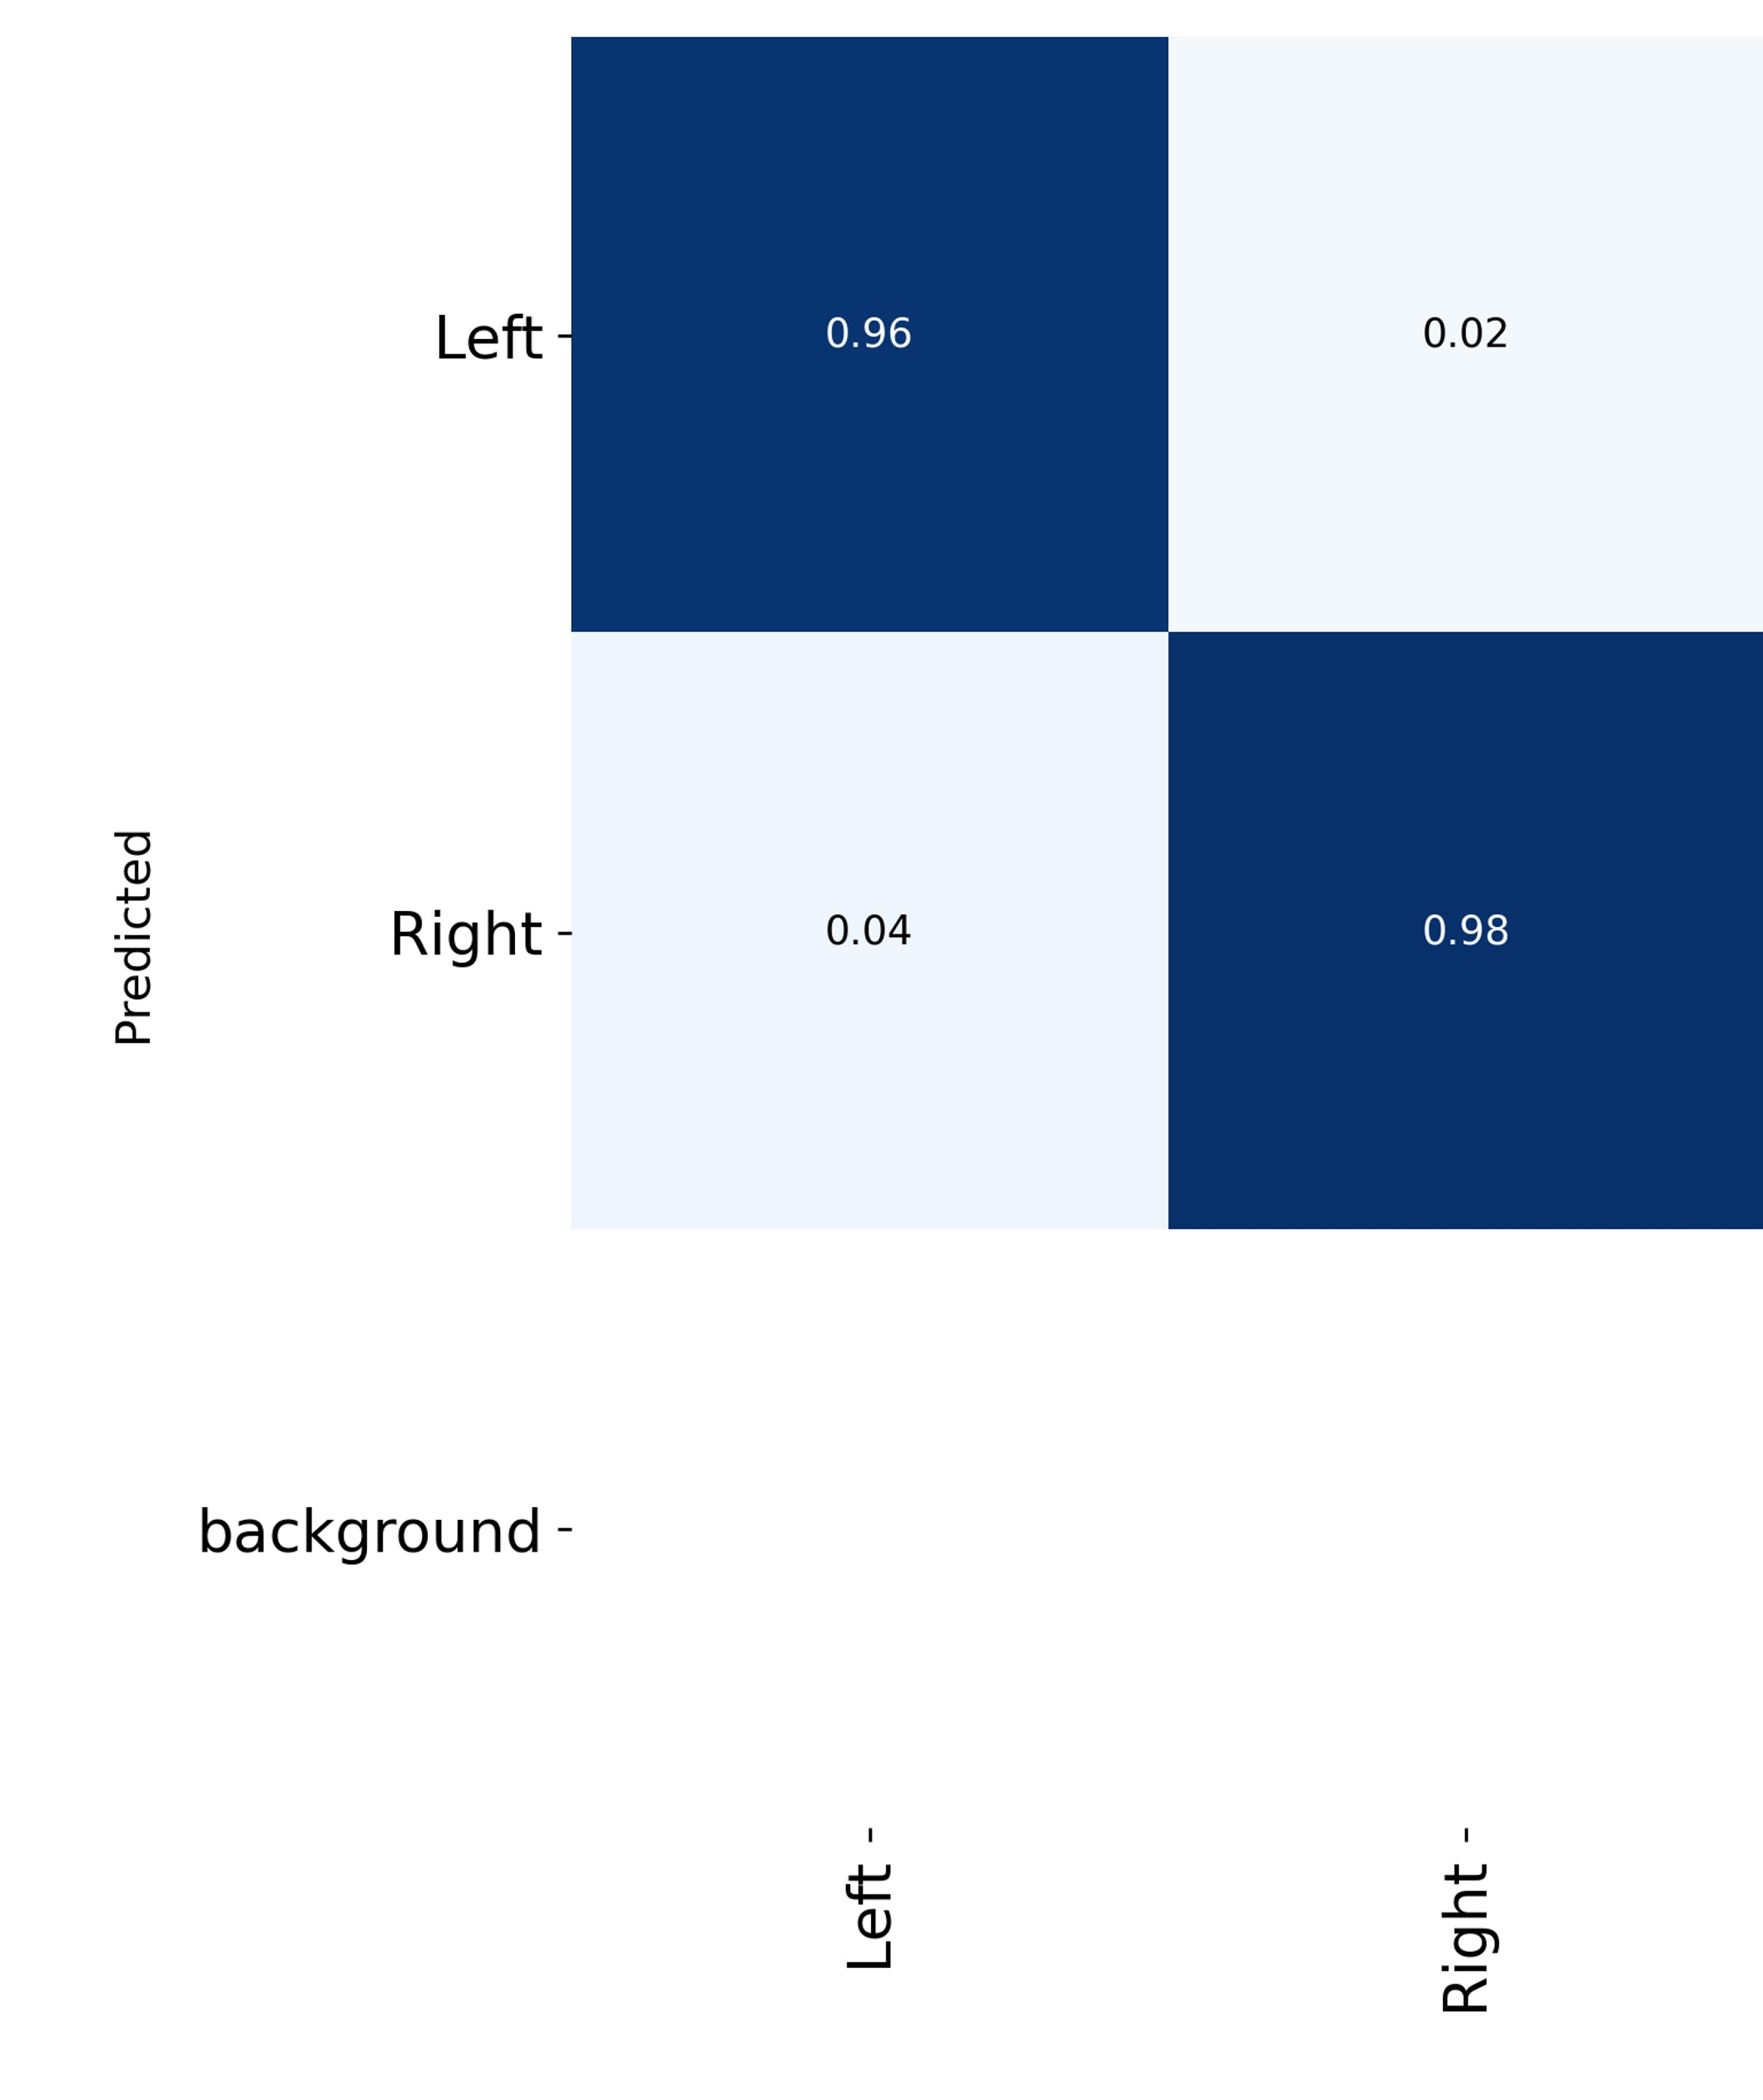
\includegraphics[width=0.7\linewidth]{conf_matr}
    \caption{Normalisierte Confusion-Matrix des Trainings}\label{conf_matr}
\end{figure}

Dabei sind auf der X-Achse die gelabelten Bounding Boxen und auf der Y-Achse die erkannten Bounding Boxen (predictions) der Klassen aufgetragen.
Hier können Korrelationen der Klassen beziehungsweise problematische Konfusionen erkannt werden.
\cite{yolo_metrics}
\newPar
Dem speziellen Beispiel kann beispielsweise entnommen werden, dass 96\% der als \textit{Left} gelabelten Objekte und 98\% der als \textit{Right}
gelabelten Objekte auch als solche erkannt werden.
\newPar
Umfangreichere Einblicke in den Trainingsvorgang sowie die \hyp{}qualität bietet die Ergebnisübersicht.

\begin{figure}[H]
    \centering
    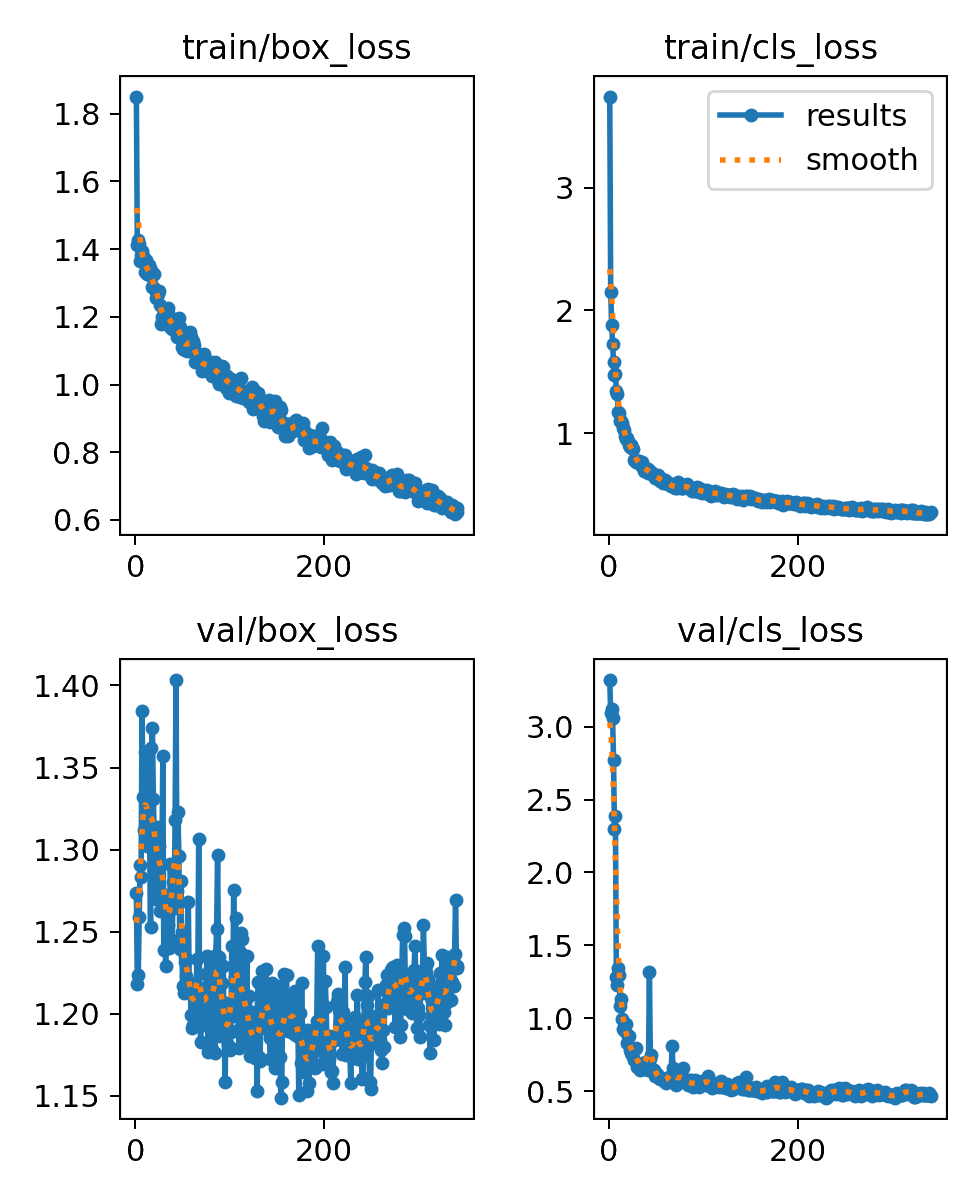
\includegraphics[width=0.6\linewidth]{results}
    \caption{Auschnitt der Ergebnisübersicht des Trainings}\label{results}
\end{figure}

Die in \imageref{results} dargestellten Graphen zum Box-Loss \textit{box\_loss} und zum Klassifikationsverlust \textit{cls\_loss} zeigen den Verlauf dieser beiden zentralen Fehlerfunktionen während des Trainings 
und der Validierung des Modells über die etwa 300 Epochen des Trainings. Die obere Reihe bezieht sich dabei auf die Trainings\hyp{} und die untere auf die Validierungsdaten.
Beide Diagramme erlauben Rückschlüsse auf die Lernfortschritte des Modells und dessen Fähigkeit, die Trainingsdaten korrekt zu verarbeiten und auf unbekannte Daten anzuwenden.
\newPar
Beim Box-Loss handelt es sich um den Fehler, den das Modell bei der Vorhersage der Position und Größe der Objekte macht. 
Im Trainingsverlauf ist ein klarer Rückgang des Box-Loss-Werts von anfangs etwa 1,8 auf unter 0,7 erkennbar. 
Dies deutet darauf hin, dass das Modell zunehmend lernt, die Objekte räumlich korrekt zu lokalisieren. 
Die Abnahme erfolgt kontinuierlich und ohne größere Schwankungen, was für ein stabiles Lernverhalten spricht. 
Im Validierungsdiagramm ist zunächst ebenfalls ein Rückgang zu erkennen, gefolgt von einem leichten Anstieg gegen Ende des Trainings. 
Dieser Verlauf kann ein Hinweis darauf sein, dass das Modell beginnt, sich zu stark an die Trainingsdaten anzupassen.
Also das oben bereits erwähnte sogenannte Overfitting.
\newPar
Der Klassifikationsverlust (\textit{cls\_loss}) beschreibt, wie gut das Modell die erkannten Objekte der richtigen Klasse zuordnet. 
Auch hier zeigt sich im Trainingsverlauf ein starker Rückgang des Fehlers, insbesondere in den frühen Epochen, gefolgt von einer langsamen Annäherung an einen stabilen Wert um 0,6. 
Das bedeutet, dass das Modell sehr schnell die grundlegenden Klassifizierungsregeln erlernt und sich dann zunehmend feiner an die Daten anpasst. 
Auf dem Validierungsdatensatz ist dieser Trend ebenfalls sichtbar, jedoch mit stärkeren Schwankungen. 
Trotzdem bleibt der Verlauf weitgehend stabil, was auf eine solide Inferenz des Modells schließen lässt.
\cite{yolo_metrics}
\newPar
Insgesamt zeigen beide Metriken, dass das Modell im Training effektiv lernt. 
Die klare Abnahme der Verluste und das weitgehend parallele Verhalten auf Trainings- und Validierungsdaten sprechen für einen erfolgreichen Optimierungsprozess, 
auch wenn sich gegen Ende eine mögliche Überanpassung andeutet.